%!TEX program = xelatex

\documentclass[a4paper, openany, oneside]{memoir}
\usepackage[no-math]{fontspec}
\usepackage{pgfplots}
\pgfplotsset{compat=newest}
\usepackage{commath}
\usepackage{mathtools}
\usepackage{amssymb}
\usepackage{amsthm}
\usepackage{booktabs}
\usepackage{mathtools}
\usepackage{xcolor}
\usepackage[separate-uncertainty=true, per-mode=symbol]{siunitx}
\usepackage[noabbrev, capitalize]{cleveref}
\usepackage{listings}
\usepackage[american inductor, european resistor]{circuitikz}
\usepackage{amsmath}
\usepackage{amsfonts}
\usepackage{ifxetex}
\usepackage[dutch,english]{babel}
\usepackage[backend=bibtexu,texencoding=utf8,bibencoding=utf8,style=ieee,sortlocale=en_GB,language=auto]{biblatex}
\usepackage[strict,autostyle]{csquotes}
\usepackage{parskip}
\usepackage{import}
\usepackage{standalone}
\usepackage{hyperref}
%\usepackage[toc,title,titletoc]{appendix}

\ifxetex{} % Fonts laden in het geval dat je met Xetex compiled
    \usepackage{fontspec}
    \defaultfontfeatures{Ligatures=TeX} % To support LaTeX quoting style
    \setromanfont{Palatino Linotype} % Tover ergens in Font mapje in root.
    \setmonofont{Source Code Pro}
\else % Terug val in standaard pdflatex tool chain. Geen ondersteuning voor OTT fonts
    \usepackage[T1]{fontenc}
    \usepackage[utf8]{inputenc}
\fi
\newcommand{\references}[1]{\begin{flushright}{#1}\end{flushright}}
\renewcommand{\vec}[1]{\boldsymbol{\mathbf{#1}}}
\newcommand{\uvec}[1]{\boldsymbol{\hat{\vec{#1}}}}
\newcommand{\mat}[1]{\boldsymbol{\mathbf{#1}}}
\newcommand{\fasor}[1]{\boldsymbol{\tilde{\vec{#1}}}}
\newcommand{\cmplx}[0]{\mathrm{j}}
\renewcommand{\Re}[0]{\operatorname{Re}}
\newcommand{\Cov}{\operatorname{Cov}}
\newcommand{\Var}{\operatorname{Var}}
\newcommand{\proj}{\operatorname{proj}}
\newcommand{\Perp}{\operatorname{perp}}
\newcommand{\col}{\operatorname{col}}
\newcommand{\rect}{\operatorname{rect}}
\newcommand{\sinc}{\operatorname{sinc}}
\newcommand{\IT}{\operatorname{IT}}
\newcommand{\F}{\mathcal{F}}

\newtheorem{definition}{Definition}
\newtheorem{theorem}{Theorem}


\DeclareSIUnit{\voltampere}{VA} %apparent power
\DeclareSIUnit{\pii}{\ensuremath{\pi}}

\hypersetup{%setup hyperlinks
    colorlinks,
    citecolor=black,
    filecolor=black,
    linkcolor=black,
    urlcolor=black
}

% Example boxes
\usepackage{fancybox}
\usepackage{framed}
\usepackage{adjustbox}
\newenvironment{simpages}%
{\AtBeginEnvironment{itemize}{\parskip=0pt\parsep=0pt\partopsep=0pt}
\def\FrameCommand{\fboxsep=.5\FrameSep\shadowbox}\MakeFramed{\FrameRestore}}%
{\endMakeFramed}

% Impulse train
\DeclareFontFamily{U}{wncy}{}
\DeclareFontShape{U}{wncy}{m}{n}{<->wncyr10}{}
\DeclareSymbolFont{mcy}{U}{wncy}{m}{n}
\DeclareMathSymbol{\Sha}{\mathord}{mcy}{"58}
\addbibresource{../../../includes/bibliography.bib}

\title{Compressive Sensing - An Overview}

\author{W.P. Bruinsma \and R.P. Hes \and H.J.C. Kroep \and T.C. Leliveld \and W.M. Melching \and T.A. aan de Wiel}

\raggedbottom

\begin{document}
\chapter{Performance}
\label{cha:performance}
In this chapter the performance of the implementation will be discussed. First we will introduce the measurements done to evaluate said performance and then we will discuss some practical implementations of these optimalisations.

\section{Profiling}
\label{sec:performance-profiling}
A good measurement technique for performance are profiling reports. Profiling reports describe the time spent inside functions. These allow us to identify bottlenecks in the system which slow down calculations. More then often these have allowed us to make crucial speed ups in the system.

\section{Algorithms and Data structures}
Our initial step was to improve the algorithms and data structures involved. This is usually seen as the first best way of improving performance. We used profiling reports as a guideline to identify bottlenecks and improve the algorithms or data structures only there were necessary as to keep the complexity of our code low\footnote{As Donald Knuth once said: ``The root of all evil is premature optimization''. The essence of this quote is that one should only start optimizing code once it has been proven to be necessary as this usually increases the complexity of the code and thus the maintainability. Maintainability is often only an afterthought but imminent for code that has to last.}.

\subsection{Sparse matrices}
\label{sec:sparse-matrices}
After the initial profiling reports it became clear that the dot product with the pseudo-inverse in the reconstructor formed a bottleneck. After doing some inspection it appeared that his matrix was sparse. The sparsity fitted good into \lib{SciPy's} sparse data structure. We chose for the rather standard \func{csr\_matrix}. As noted by \cite{scipy} the advantages of this data structure are amongst other fast matrix vector products and better memory efficiency. The speed difference for the reconstruct method is shown in \cref{fig:sparse}.

\begin{figure}[]
    \centering
    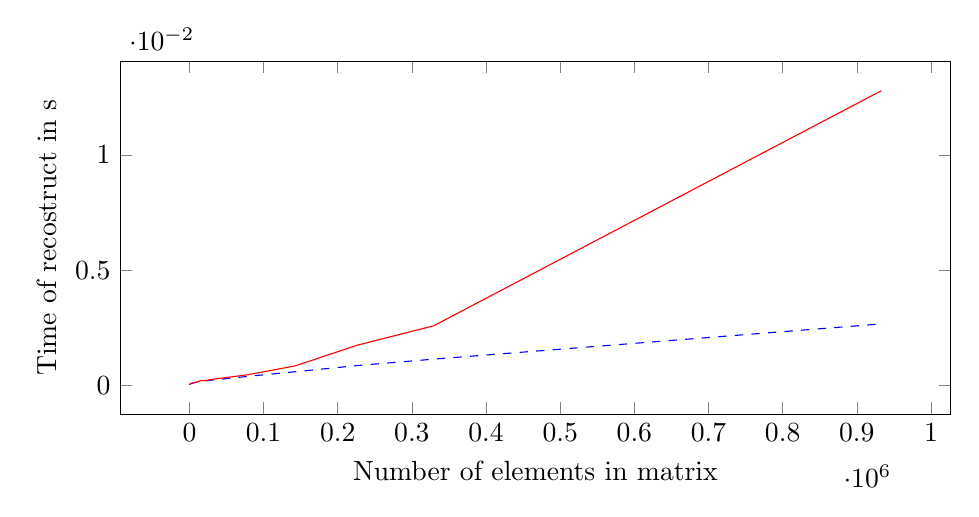
\begin{tikzpicture}
    \begin{axis}[%
        width=\linewidth,
        height=0.5\linewidth,
        xlabel={Number of elements in matrix},
        ylabel={Time of recostruct in \si{s}},
        ]
        \addplot [
        color=blue,
        dashed,
        ]
        table[col sep=comma]{
1.600000000000000000e+01,2.280402183532714977e-05
6.240000000000000000e+02,4.161381721496581955e-05
2.000000000000000000e+03,6.225585937500000108e-05
4.144000000000000000e+03,8.629393577575683203e-05
7.056000000000000000e+03,1.075601577758789030e-04
1.073600000000000000e+04,1.289680004119873142e-04
1.518400000000000000e+04,1.560301780700683566e-04
2.040000000000000000e+04,1.757450103759765727e-04
2.638400000000000000e+04,2.060890197753906196e-04
3.313600000000000000e+04,2.274580001831054735e-04
7.841600000000000000e+04,3.817260265350341905e-04
1.428960000000000000e+05,5.848600864410400703e-04
2.265760000000000000e+05,8.532679080963134245e-04
3.294560000000000000e+05,1.131367921829223725e-03
9.329760000000000000e+05,2.661290168762207083e-03
};
        \addplot [
        color=red,
        solid,
        ]
        table[col sep=comma]{
1.600000000000000000e+01,1.751399040222168045e-05
6.240000000000000000e+02,5.141210556030273562e-05
2.000000000000000000e+03,8.130097389221190842e-05
4.144000000000000000e+03,9.130501747131347960e-05
7.056000000000000000e+03,1.178588867187500030e-04
1.073600000000000000e+04,1.449580192565918082e-04
1.518400000000000000e+04,2.048060894012451185e-04
2.040000000000000000e+04,1.967520713806152478e-04
2.638400000000000000e+04,2.263691425323486358e-04
3.313600000000000000e+04,2.653179168701172040e-04
7.841600000000000000e+04,4.512910842895508025e-04
1.428960000000000000e+05,8.393068313598632795e-04
2.265760000000000000e+05,1.739547014236450268e-03
3.294560000000000000e+05,2.581127166748046695e-03
9.329760000000000000e+05,1.279244780540466329e-02
};
\end{axis}
\end{tikzpicture}

    \caption{Time of reconstruct (normalized over 1000 runs) versus number of elements in matrix of sparse (dashed) and standard matrix (solid) data structure}
    \label{fig:sparse}
\end{figure}

\subsection{Vectorisation}
\label{sec:vectorisation}
Another bottleneck that was observed were the signal cross correlations. There are a number of ways to calculate it namely:
\begin{itemize}
    \item Cross correlations written out as a number of matrix multiplications,
    \item \lib{Numpy's} \func{correlate} function, and
    \item \lib{SciPy's} \func{fftconvolve} function.
\end{itemize}
As can be seen in \cref{fig:sparse} each technique has its own area of best performance. The matrix multiplication is best until a vector length of about 50. \lib{Numpy's} \func{Correlate} is the best from 50 until 400 and for everything above that \func{fftconvolve} is the fastest.

\begin{figure}[]
    \centering
    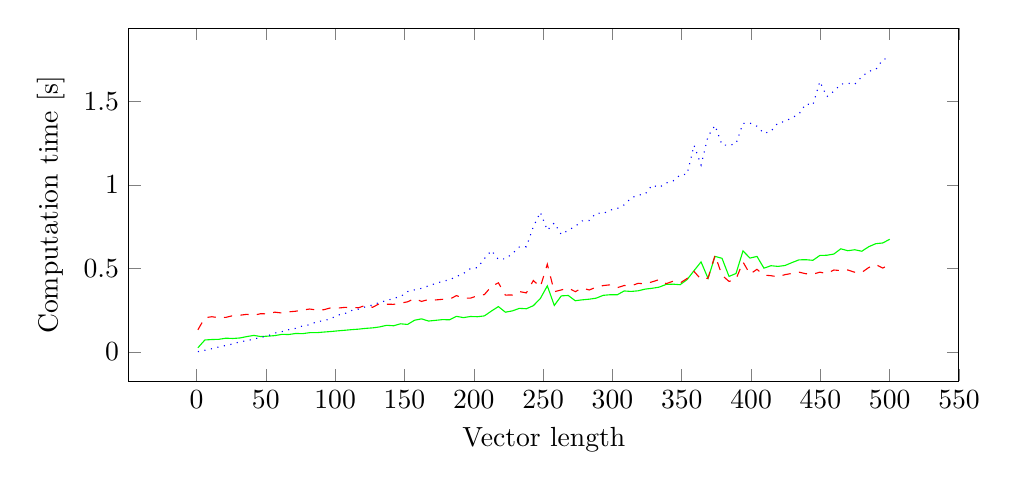
\begin{tikzpicture}
    \begin{axis}[%
        width=\linewidth,
        height=0.5\linewidth,
        xlabel={Vector length},
        ylabel={Computation time [\si{s}]},
        ]
        \addplot [
        color=green,
        solid,
        ]
        table[col sep=comma]{
1.000000000000000000e+00,2.511096000671386719e-02
6.040404040404040664e+00,7.164287567138671875e-02
1.108080808080808133e+01,7.437610626220703125e-02
1.612121212121212110e+01,7.565689086914062500e-02
2.116161616161616266e+01,8.236908912658691406e-02
2.620202020202020421e+01,8.062791824340820312e-02
3.124242424242424221e+01,8.367586135864257812e-02
3.628282828282828376e+01,9.197711944580078125e-02
4.132323232323232531e+01,9.913897514343261719e-02
4.636363636363636687e+01,9.206104278564453125e-02
5.140404040404040842e+01,9.459805488586425781e-02
5.644444444444444997e+01,9.767913818359375000e-02
6.148484848484848442e+01,1.052420139312744141e-01
6.652525252525252597e+01,1.044139862060546875e-01
7.156565656565656752e+01,1.106150150299072266e-01
7.660606060606060908e+01,1.095860004425048828e-01
8.164646464646465063e+01,1.154642105102539062e-01
8.668686868686869218e+01,1.153070926666259766e-01
9.172727272727273373e+01,1.190440654754638672e-01
9.676767676767677528e+01,1.221780776977539062e-01
1.018080808080808168e+02,1.261851787567138672e-01
1.068484848484848584e+02,1.297111511230468750e-01
1.118888888888888999e+02,1.334559917449951172e-01
1.169292929292929415e+02,1.365590095520019531e-01
1.219696969696969688e+02,1.410980224609375000e-01
1.270101010101010104e+02,1.440579891204833984e-01
1.320505050505050519e+02,1.497950553894042969e-01
1.370909090909090935e+02,1.593589782714843750e-01
1.421313131313131350e+02,1.567499637603759766e-01
1.471717171717171766e+02,1.685280799865722656e-01
1.522121212121212182e+02,1.646239757537841797e-01
1.572525252525252597e+02,1.898391246795654297e-01
1.622929292929293013e+02,1.980960369110107422e-01
1.673333333333333428e+02,1.849257946014404297e-01
1.723737373737373844e+02,1.891419887542724609e-01
1.774141414141414259e+02,1.935629844665527344e-01
1.824545454545454675e+02,1.923749446868896484e-01
1.874949494949495090e+02,2.131960391998291016e-01
1.925353535353535506e+02,2.054369449615478516e-01
1.975757575757575921e+02,2.121529579162597656e-01
2.026161616161616337e+02,2.108240127563476562e-01
2.076565656565656752e+02,2.158350944519042969e-01
2.126969696969697168e+02,2.447941303253173828e-01
2.177373737373737583e+02,2.715160846710205078e-01
2.227777777777777999e+02,2.379400730133056641e-01
2.278181818181818414e+02,2.457430362701416016e-01
2.328585858585858830e+02,2.608501911163330078e-01
2.378989898989899245e+02,2.585990428924560547e-01
2.429393939393939377e+02,2.769041061401367188e-01
2.479797979797979792e+02,3.196630477905273438e-01
2.530202020202020208e+02,3.953819274902343750e-01
2.580606060606060623e+02,2.782721519470214844e-01
2.631010101010101039e+02,3.356699943542480469e-01
2.681414141414141454e+02,3.379421234130859375e-01
2.731818181818181870e+02,3.065800666809082031e-01
2.782222222222222285e+02,3.118848800659179688e-01
2.832626262626262701e+02,3.157389163970947266e-01
2.883030303030303116e+02,3.219580650329589844e-01
2.933434343434343532e+02,3.388788700103759766e-01
2.983838383838383947e+02,3.423850536346435547e-01
3.034242424242424363e+02,3.419840335845947266e-01
3.084646464646464779e+02,3.649890422821044922e-01
3.135050505050505194e+02,3.621308803558349609e-01
3.185454545454545610e+02,3.659150600433349609e-01
3.235858585858586025e+02,3.760769367218017578e-01
3.286262626262626441e+02,3.810110092163085938e-01
3.336666666666666856e+02,3.878121376037597656e-01
3.387070707070707272e+02,4.039969444274902344e-01
3.437474747474747687e+02,4.055778980255126953e-01
3.487878787878788103e+02,4.024000167846679688e-01
3.538282828282828518e+02,4.328281879425048828e-01
3.588686868686868934e+02,4.867770671844482422e-01
3.639090909090909349e+02,5.389270782470703125e-01
3.689494949494949765e+02,4.403932094573974609e-01
3.739898989898990180e+02,5.718820095062255859e-01
3.790303030303030596e+02,5.603299140930175781e-01
3.840707070707071011e+02,4.520008563995361328e-01
3.891111111111111427e+02,4.694690704345703125e-01
3.941515151515151842e+02,6.047310829162597656e-01
3.991919191919192258e+02,5.616359710693359375e-01
4.042323232323232673e+02,5.717291831970214844e-01
4.092727272727273089e+02,5.013351440429687500e-01
4.143131313131313505e+02,5.159971714019775391e-01
4.193535353535353920e+02,5.119907855987548828e-01
4.243939393939394336e+02,5.171461105346679688e-01
4.294343434343434751e+02,5.345411300659179688e-01
4.344747474747475167e+02,5.510299205780029297e-01
4.395151515151515582e+02,5.520660877227783203e-01
4.445555555555555998e+02,5.483589172363281250e-01
4.495959595959596413e+02,5.775690078735351562e-01
4.546363636363636829e+02,5.785939693450927734e-01
4.596767676767677244e+02,5.858519077301025391e-01
4.647171717171717660e+02,6.172339916229248047e-01
4.697575757575758075e+02,6.058561801910400391e-01
4.747979797979798491e+02,6.114790439605712891e-01
4.798383838383838906e+02,6.026659011840820312e-01
4.848787878787878753e+02,6.299340724945068359e-01
4.899191919191919169e+02,6.478559970855712891e-01
4.949595959595959584e+02,6.521608829498291016e-01
5.000000000000000000e+02,6.742269992828369141e-01
};
        \addplot [
        color=red,
        dashed,
        ]
        table[col sep=comma]{
            1.000000000000000000e+00,1.325831413269042969e-01
            6.040404040404040664e+00,2.048919200897216797e-01
            1.108080808080808133e+01,2.107329368591308594e-01
            1.612121212121212110e+01,2.046349048614501953e-01
            2.116161616161616266e+01,2.069840431213378906e-01
            2.620202020202020421e+01,2.171480655670166016e-01
            3.124242424242424221e+01,2.197048664093017578e-01
            3.628282828282828376e+01,2.251350879669189453e-01
            4.132323232323232531e+01,2.198779582977294922e-01
            4.636363636363636687e+01,2.289381027221679688e-01
            5.140404040404040842e+01,2.277019023895263672e-01
            5.644444444444444997e+01,2.382419109344482422e-01
            6.148484848484848442e+01,2.331581115722656250e-01
            6.652525252525252597e+01,2.400510311126708984e-01
            7.156565656565656752e+01,2.437050342559814453e-01
            7.660606060606060908e+01,2.508289813995361328e-01
            8.164646464646465063e+01,2.569000720977783203e-01
            8.668686868686869218e+01,2.509820461273193359e-01
            9.172727272727273373e+01,2.525291442871093750e-01
            9.676767676767677528e+01,2.638759613037109375e-01
            1.018080808080808168e+02,2.625570297241210938e-01
            1.068484848484848584e+02,2.664849758148193359e-01
            1.118888888888888999e+02,2.658810615539550781e-01
            1.169292929292929415e+02,2.645409107208251953e-01
            1.219696969696969688e+02,2.792727947235107422e-01
            1.270101010101010104e+02,2.671868801116943359e-01
            1.320505050505050519e+02,2.895681858062744141e-01
            1.370909090909090935e+02,2.858550548553466797e-01
            1.421313131313131350e+02,2.849359512329101562e-01
            1.471717171717171766e+02,2.921900749206542969e-01
            1.522121212121212182e+02,2.999019622802734375e-01
            1.572525252525252597e+02,3.195490837097167969e-01
            1.622929292929293013e+02,3.023819923400878906e-01
            1.673333333333333428e+02,3.138680458068847656e-01
            1.723737373737373844e+02,3.112139701843261719e-01
            1.774141414141414259e+02,3.150360584259033203e-01
            1.824545454545454675e+02,3.156130313873291016e-01
            1.874949494949495090e+02,3.371930122375488281e-01
            1.925353535353535506e+02,3.219192028045654297e-01
            1.975757575757575921e+02,3.220100402832031250e-01
            2.026161616161616337e+02,3.363959789276123047e-01
            2.076565656565656752e+02,3.433439731597900391e-01
            2.126969696969697168e+02,3.925390243530273438e-01
            2.177373737373737583e+02,4.138569831848144531e-01
            2.227777777777777999e+02,3.401780128479003906e-01
            2.278181818181818414e+02,3.411171436309814453e-01
            2.328585858585858830e+02,3.614530563354492188e-01
            2.378989898989899245e+02,3.533768653869628906e-01
            2.429393939393939377e+02,4.274370670318603516e-01
            2.479797979797979792e+02,3.889207839965820312e-01
            2.530202020202020208e+02,5.250248908996582031e-01
            2.580606060606060623e+02,3.606369495391845703e-01
            2.631010101010101039e+02,3.711211681365966797e-01
            2.681414141414141454e+02,3.821039199829101562e-01
            2.731818181818181870e+02,3.609130382537841797e-01
            2.782222222222222285e+02,3.824119567871093750e-01
            2.832626262626262701e+02,3.707928657531738281e-01
            2.883030303030303116e+02,3.879220485687255859e-01
            2.933434343434343532e+02,3.971819877624511719e-01
            2.983838383838383947e+02,4.017639160156250000e-01
            3.034242424242424363e+02,3.843588829040527344e-01
            3.084646464646464779e+02,3.976140022277832031e-01
            3.135050505050505194e+02,3.956959247589111328e-01
            3.185454545454545610e+02,4.107718467712402344e-01
            3.235858585858586025e+02,4.076650142669677734e-01
            3.286262626262626441e+02,4.194178581237792969e-01
            3.336666666666666856e+02,4.328238964080810547e-01
            3.387070707070707272e+02,4.085040092468261719e-01
            3.437474747474747687e+02,4.233639240264892578e-01
            3.487878787878788103e+02,4.124689102172851562e-01
            3.538282828282828518e+02,4.394099712371826172e-01
            3.588686868686868934e+02,4.815080165863037109e-01
            3.639090909090909349e+02,4.343609809875488281e-01
            3.689494949494949765e+02,4.416589736938476562e-01
            3.739898989898990180e+02,5.789680480957031250e-01
            3.790303030303030596e+02,4.585790634155273438e-01
            3.840707070707071011e+02,4.221129417419433594e-01
            3.891111111111111427e+02,4.354329109191894531e-01
            3.941515151515151842e+02,5.386009216308593750e-01
            3.991919191919192258e+02,4.657740592956542969e-01
            4.042323232323232673e+02,4.943981170654296875e-01
            4.092727272727273089e+02,4.598538875579833984e-01
            4.143131313131313505e+02,4.563119411468505859e-01
            4.193535353535353920e+02,4.496819972991943359e-01
            4.243939393939394336e+02,4.626400470733642578e-01
            4.294343434343434751e+02,4.698979854583740234e-01
            4.344747474747475167e+02,4.775791168212890625e-01
            4.395151515151515582e+02,4.680299758911132812e-01
            4.445555555555555998e+02,4.648489952087402344e-01
            4.495959595959596413e+02,4.775538444519042969e-01
            4.546363636363636829e+02,4.686031341552734375e-01
            4.596767676767677244e+02,4.903519153594970703e-01
            4.647171717171717660e+02,4.869501590728759766e-01
            4.697575757575758075e+02,4.907188415527343750e-01
            4.747979797979798491e+02,4.768421649932861328e-01
            4.798383838383838906e+02,4.756669998168945312e-01
            4.848787878787878753e+02,5.054700374603271484e-01
            4.899191919191919169e+02,5.230388641357421875e-01
            4.949595959595959584e+02,5.016658306121826172e-01
            5.000000000000000000e+02,5.251190662384033203e-01
};
\addplot [
    color=blue,
    dotted,
        ]
        table[col sep=comma]{
1.000000000000000000e+00,1.729011535644531250e-03
6.040404040404040664e+00,1.044011116027832031e-02
1.108080808080808133e+01,1.951694488525390625e-02
1.612121212121212110e+01,2.979898452758789062e-02
2.116161616161616266e+01,3.897190093994140625e-02
2.620202020202020421e+01,4.776310920715332031e-02
3.124242424242424221e+01,6.091809272766113281e-02
3.628282828282828376e+01,6.741809844970703125e-02
4.132323232323232531e+01,7.712793350219726562e-02
4.636363636363636687e+01,8.734917640686035156e-02
5.140404040404040842e+01,9.637784957885742188e-02
5.644444444444444997e+01,1.130211353302001953e-01
6.148484848484848442e+01,1.212520599365234375e-01
6.652525252525252597e+01,1.335520744323730469e-01
7.156565656565656752e+01,1.413350105285644531e-01
7.660606060606060908e+01,1.564378738403320312e-01
8.164646464646465063e+01,1.630351543426513672e-01
8.668686868686869218e+01,1.807770729064941406e-01
9.172727272727273373e+01,1.870629787445068359e-01
9.676767676767677528e+01,1.981010437011718750e-01
1.018080808080808168e+02,2.203540802001953125e-01
1.068484848484848584e+02,2.289860248565673828e-01
1.118888888888888999e+02,2.482059001922607422e-01
1.169292929292929415e+02,2.562489509582519531e-01
1.219696969696969688e+02,2.702970504760742188e-01
1.270101010101010104e+02,2.813417911529541016e-01
1.320505050505050519e+02,2.970709800720214844e-01
1.370909090909090935e+02,3.070600032806396484e-01
1.421313131313131350e+02,3.209679126739501953e-01
1.471717171717171766e+02,3.311460018157958984e-01
1.522121212121212182e+02,3.611378669738769531e-01
1.572525252525252597e+02,3.712611198425292969e-01
1.622929292929293013e+02,3.804728984832763672e-01
1.673333333333333428e+02,3.956809043884277344e-01
1.723737373737373844e+02,4.093461036682128906e-01
1.774141414141414259e+02,4.228620529174804688e-01
1.824545454545454675e+02,4.317131042480468750e-01
1.874949494949495090e+02,4.513740539550781250e-01
1.925353535353535506e+02,4.693360328674316406e-01
1.975757575757575921e+02,4.990620613098144531e-01
2.026161616161616337e+02,5.044310092926025391e-01
2.076565656565656752e+02,5.586469173431396484e-01
2.126969696969697168e+02,6.070380210876464844e-01
2.177373737373737583e+02,5.538029670715332031e-01
2.227777777777777999e+02,5.578219890594482422e-01
2.278181818181818414e+02,5.878601074218750000e-01
2.328585858585858830e+02,6.284470558166503906e-01
2.378989898989899245e+02,6.294419765472412109e-01
2.429393939393939377e+02,7.488648891448974609e-01
2.479797979797979792e+02,8.361380100250244141e-01
2.530202020202020208e+02,7.279798984527587891e-01
2.580606060606060623e+02,7.720749378204345703e-01
2.631010101010101039e+02,7.024581432342529297e-01
2.681414141414141454e+02,7.287080287933349609e-01
2.731818181818181870e+02,7.517440319061279297e-01
2.782222222222222285e+02,7.845160961151123047e-01
2.832626262626262701e+02,7.868349552154541016e-01
2.883030303030303116e+02,8.313140869140625000e-01
2.933434343434343532e+02,8.275971412658691406e-01
2.983838383838383947e+02,8.489260673522949219e-01
3.034242424242424363e+02,8.580720424652099609e-01
3.084646464646464779e+02,8.804199695587158203e-01
3.135050505050505194e+02,9.215888977050781250e-01
3.185454545454545610e+02,9.385960102081298828e-01
3.235858585858586025e+02,9.441471099853515625e-01
3.286262626262626441e+02,9.990239143371582031e-01
3.336666666666666856e+02,9.843468666076660156e-01
3.387070707070707272e+02,1.011020183563232422e+00
3.437474747474747687e+02,1.023281812667846680e+00
3.487878787878788103e+02,1.059054136276245117e+00
3.538282828282828518e+02,1.064209938049316406e+00
3.588686868686868934e+02,1.236235141754150391e+00
3.639090909090909349e+02,1.118686914443969727e+00
3.689494949494949765e+02,1.290804862976074219e+00
3.739898989898990180e+02,1.355365991592407227e+00
3.790303030303030596e+02,1.239078044891357422e+00
3.840707070707071011e+02,1.236415863037109375e+00
3.891111111111111427e+02,1.245979070663452148e+00
3.941515151515151842e+02,1.367418050765991211e+00
3.991919191919192258e+02,1.369467973709106445e+00
4.042323232323232673e+02,1.350603818893432617e+00
4.092727272727273089e+02,1.307971954345703125e+00
4.143131313131313505e+02,1.320370912551879883e+00
4.193535353535353920e+02,1.369797945022583008e+00
4.243939393939394336e+02,1.379172086715698242e+00
4.294343434343434751e+02,1.401427030563354492e+00
4.344747474747475167e+02,1.422371149063110352e+00
4.395151515151515582e+02,1.484793901443481445e+00
4.445555555555555998e+02,1.477195978164672852e+00
4.495959595959596413e+02,1.618315935134887695e+00
4.546363636363636829e+02,1.527771949768066406e+00
4.596767676767677244e+02,1.559514999389648438e+00
4.647171717171717660e+02,1.602515935897827148e+00
4.697575757575758075e+02,1.607869863510131836e+00
4.747979797979798491e+02,1.602185964584350586e+00
4.798383838383838906e+02,1.646977901458740234e+00
4.848787878787878753e+02,1.679275989532470703e+00
4.899191919191919169e+02,1.689788818359375000e+00
4.949595959595959584e+02,1.749567031860351562e+00
5.000000000000000000e+02,1.761135101318359375e+00
};

\end{axis}
\end{tikzpicture}

    \caption{Time to do 100 cross-correlations plot against the size of the vector. Solid is NumPy's correlate, dashed is SciPy's fftconvolve and dotted is the matrix implementation.}
    \label{fig:sparse}
\end{figure}

\section{Multiprocessing}
\label{sec:multiprocessing}

Each major part of the model (source, sampling, reconstruction and detection) can be run simultaneously by means of implementing a pipeline. This is done by the means of multiprocessing. We spawn a separate process for each part and pass the information around using inter-process communication. This introduces some overhead and delay because of the IPC but has the major advantage of allowing us to make use of more cores on the CPU. Ultimately it depends on the configuration of the parameters whether multiprocessing is advantageous, because the IPC (which has to do memory transfers through L3) can be the bottleneck on less demanding parameter sets.

%TODO Nog eens goed multiprocessing vs andere zwets bekijken
\section{Results \& Improvements}
\label{sec:results}
%TODO refresh rate constructor
\end{document}
